\documentclass[version=last,fontsize=12pt, parskip=full-]{scrartcl}
\usepackage{polyglossia}
\setdefaultlanguage{english}
\setotherlanguage{german}
\setmainfont{Barlow}
\setsansfont{Barlow}
\newfontfamily\NotoSans{Noto Sans}

\usepackage{geometry}
\geometry{
  width=210mm,
  height=297mm,
  %portrait,
  top=20mm,
  left=20mm,
  right=20mm,
  bottom=25mm,
  headsep=3mm,
  footskip=12mm
}
\usepackage{ragged2e} % nicer typesetting (hyphenation) for non raggedright and raggedleft
\usepackage[]{microtype}
\usepackage[manualmark]{scrlayer-scrpage}
\newpairofpagestyles[]{nothing}{}

\usepackage{graphicx} % graphics
\usepackage[table]{xcolor}

\usepackage{tikz}
\usetikzlibrary{calc}

\definecolor{ochsenblutrot}{HTML}{59191F}
\definecolor{tramstop}{HTML}{4255B3}

\newcommand{\bilingual}[2]{#1 \textgerman{\emph{#2}}}
\newcommand{\bilingualHeading}[2]{\textbf{#1} \textgerman{\emph{#2}}}
\newcommand{\bilingualLinebreak}[2]{#1\newline \textgerman{\emph{#2}}}
\newcommand{\largeSpace}{\vspace{0.5\baselineskip}}

\begin{document}
\pagestyle{nothing}
\selectlanguage{english}

\chead{\bilingual{\small Print out on A4 paper.}{\small Bitte auf A4 ausdrucken.}}

{
  \Huge
  \textbf{Your Ticket}
}
{
  \Large
  \emph{Ihr Ticket}
}

\newlength\titleRightBoxWidth
\setlength{\titleRightBoxWidth}{\linewidth}
\newlength\titleLeftBoxWidth
\setlength{\titleLeftBoxWidth}{60mm}
\advance\titleRightBoxWidth by -\titleLeftBoxWidth

\begin{tikzpicture}[x=1mm, y=1mm]
  \fill[color=ochsenblutrot, rounded corners=4mm] (0,0) rectangle (\linewidth, 30);
  \node at (15,0) [anchor=south west, inner sep=3mm] {%
    
\includegraphics[height=24mm]{images/sotm19-logo.pdf}%
  };
  \node at (55,5) [anchor=south west, inner sep=3mm] {%
    \begin{minipage}{\titleRightBoxWidth}%
      \Large
      \color{white}
      \textbf{\LARGE STATE OF THE MAP}\\
      Heidelberg, 21–23 September 2019
    \end{minipage}%
  };
\end{tikzpicture}

\renewcommand{\arraystretch}{1.6}
\newcolumntype{L}[1]{>{\RaggedRight\arraybackslash}p{#1}}
\begin{tabular}{|L{50mm}|L{40mm}|L{30mm}|L{32mm}|}
\hline
\bilingualHeading{\large Name}{Name} & \multicolumn{3}{L{100mm}|}{\large Max Christian Wilhelm Mustermanngroßbauernbergerhofner}\tabularnewline
\hline
\bilingualHeading{\large Ticket type}{Preisklasse} & \multicolumn{3}{L{100mm}|}{\large Community Early Bird}
\tabularnewline
\hline
\bilingualHeading{\large Price}{Preis} & {\large EUR 75}
& ---
& ---
\tabularnewline
\hline
\bilingualHeading{\large Organiser}{Veranstalter} & \multicolumn{3}{L{105mm}|}{OpenStreetMap Foundation, St John’s Innovation Centre, Cowley Road, Cambridge, CB4 0WS, Vereinigtes Königreich}\tabularnewline
\hline
\end{tabular}
\renewcommand{\arraystretch}{1.0}

\bilingual{\small This is not an invoice.}{\small Dies ist keine Rechnung.}

\begin{minipage}{0.55\linewidth}%
  \begin{tikzpicture}[x=1mm, y=1mm]
    \node at (0,0) [anchor=south west] {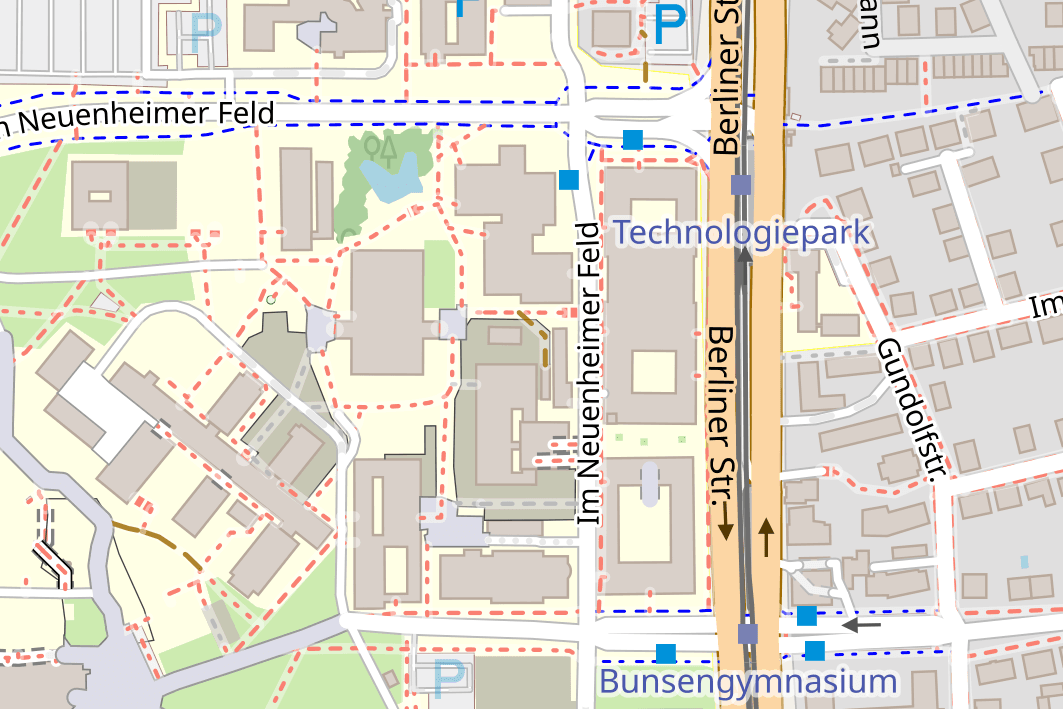
\includegraphics[height=60mm]{images/ticketkarte128-small.png}};
    \node at (34, 32) [anchor=south] {
\includegraphics[]{images/marker.png}};
    \node at (0,0) [anchor=south west, fill=white] {\tiny © OpenStreetMap contributors};
  \end{tikzpicture}
\end{minipage}
\fcolorbox{black}{white}{%
  \begin{minipage}[c][57mm][t]{0.42\linewidth}
    \RaggedRight
    \bilingualHeading{\large Location}{Veranstaltungsort}\\
    Universität Heidelberg\\
    Hörsaalzentrum Chemie\\
    Im Neuenheimer Feld 252\\
    69120 Heidelberg
  
    \largeSpace
    \bilingualHeading{\large Next tram stop}{Nächste Haltestelle}\\
    Bunsengymnasium
  
    \largeSpace
    \bilingualHeading{\large Social Event}{Abendveranstaltung}\\
    HebelHalle, Hebelstr. 9, 69115 Heidelberg
  \end{minipage}
}
\justifying

{\small This ticket includes a public transport ticket for the whole VRN area. It is
valid from 21 to 23 September 2019 on all buses, trams, S-Bahn trains and
regional trains (RB, RE, IRE). It is not valid on long distance trains (IC, EC,
ICE, TGV, RJ), night trains (NJ, EN) and Flixtrain. The ticket is only valid
together with a valid passport or equal ID card.%}
\end{document}
